% Q2 paper section. AI assistance is disclosed by the shared AIcredit macro.
\section{结构水热耦合的触发条件与机制评估}\label{q2:sec-model}

气象因素通过界面温度、裂隙储水和结构损伤作用于坡体稳定性。为区分这些传递路径，本文建立共享几何与初态的结构基础模型 S、结构加热模型 ST、结构加水模型 SH，以及结构热水耦合模型 STH。四组统一输出稳定裕度、临界水头和首次机械越阈区间，使因素关联进一步转化为可计算的力学条件。

\subsection{共同力学骨架与条件参数}\label{q2:sec-structure}

以潜在结构面上的单位面积平面板表示源区承载体。设滑面倾角为 $\theta$，法向厚度为 $h$，岩石体积分数为 $r$，均质密度为 $\rho=2700r+917(1-r)$。岩桥面积比例 $f_b$ 与整体组分 $r$ 分别描述承载结构和质量组成。法向应力 $\sigma_n$ 与驱动剪应力 $\tau_g$ 为
\begin{equation}
  \sigma_n=10^{-3}\rho gh\cos\theta,\qquad
  \tau_g=10^{-3}\rho gh\sin\theta,
  \quad g=9.80665\ \mathrm{m\,s^{-2}}.
  \label{q2:eq-stress}
\end{equation}
式中应力单位为 kPa。引入界面温度 $T$、黏聚损伤比例 $D\in[0,1)$ 和孔压 $u$，将冰填节理与岩桥的黏聚、摩擦贡献按面积混合：
\begin{equation}
\begin{aligned}
 C(T,D)&=(1-D)\{f_bc_b+(1-f_b)c_j(T)\},\\
 \mu_e(T)&=f_b\mu_b+(1-f_b)\mu_j(T),\\
 R&=C(T,D)+\max(\sigma_n-u,0)\mu_e(T),\qquad
 M=\frac{R-\tau_g}{\tau_g}.
\end{aligned}\label{q2:eq-resistance}
\end{equation}
$M>0$ 表示抗力高于驱动力，$M=0$ 为临界面。损伤只衰减黏聚项；有效应力的非负截断表示失去压接后不继续产生负摩擦抗力。

冰填节理采用 Mamot 等的快速剪切试验关系\cite{q2-mamot2018}：
\begin{equation}
 c_j(T)=53.3-73.5T\quad(\mathrm{kPa}),\qquad
 \mu_j(T)=0.42-0.21T.\label{q2:eq-strength}
\end{equation}
其实验对象为冰填石灰岩节理，温度为 $-8$ 至 $-0.5\,^{\circ}\mathrm C$、名义法向应力为 100--400 kPa，平均应变率为 $(4.8\pm1.4)\times10^{-3}\,\mathrm{s^{-1}}$。计算同时保留线性延伸和暖端岩接触两种策略；后者在 $T>-0.5\,^{\circ}\mathrm C$ 时置 $c_j=0$、$\mu_j=0.60$，用于检验接触形式变化的影响。两策略沿用同一计算引擎，实验数值域标记随状态输出。

\begin{table}[htbp]
\centering\small
\caption{共同参数设计及单位；范围用于空间填充比较，非概率先验}
\label{q2:tab-parameters}
\begin{tabularx}{\linewidth}{@{}l Y Y@{}}
\toprule
过程 & 参数及设计范围 & 参数及设计范围\\
\midrule
结构几何 & $\theta:30$--$60^{\circ}$ & $h:10$--$60\ \mathrm m$\\
组成与岩桥 & $r:0.2$--$0.8$；$f_b:0$--$0.25$ & $c_b:300$--$3000\ \mathrm{kPa}$；$\mu_b:0.45$--$0.85$\\
热初态与边界 & $T_0:-6$--$-0.8\,^{\circ}\mathrm C$ & $\Delta T:-18$--$-6\,^{\circ}\mathrm C$\\
传热路径 & $\alpha:(0.9$--$2.1)\times10^{-6}\ \mathrm{m^2/s}$ & $z:0.5$--$20\ \mathrm m$\\
储排水 & $S_y:0.002$--$0.08$；$\tau_0:3$--$240\ \mathrm h$ & $H_{\rm conn}:2$--$40\ \mathrm m$\\
水量输入 & $m_R:0.25$--$3$ & $k_m:0.5$--$6\ \mathrm{mm/(^{\circ}C\,d)}$\\
损伤演化 & $A:10^{-7}$--$2\times10^{-4}\ \mathrm{h^{-1}}$ & $n:2$--$6$；$D_0:0.05$--$0.7$；$\kappa:0$--$3$\\
\bottomrule
\end{tabularx}
\end{table}

表\ref{q2:tab-parameters}给出 19 维条件参数域。其中 $\alpha$ 的端点取自外部基岩热扩散率中位数及 MAD 范围\cite{q2-weber2025}；几何、岩桥、站源映射和水力参数用于情景对照。固定种子生成 256 个共同空间填充设计点，逐点配对四机制与两强度策略，形成 $256\times4\times2=2048$ 条情景。边界覆盖 2026 年 6 月 1 日至 8 月 27 日（UTC）的 2089 个小时状态，$W_0=0$。温度使用 QC0 观测；降水按条件小时率解释，经站源倍率和液态分配进入模型。

\subsection{热传导、储排水与损伤的状态耦合}\label{q2:sec-coupling}

令站点空气温度为 $T_a$，映射到源区的空气边界为 $T_s=T_a+\Delta T$，冰接触表面边界取 $B=\min(T_s,0)$。对常扩散率、均匀初温和一维半无限导热，本文采用分段常值边界的阶跃叠加作为线性传热数值参考：
\begin{equation}
\begin{aligned}
 T(z,t_k)&=T_0+\sum_{j<k}\Delta B_j\,
 \operatorname{erfc}\!\left(\frac{z}{2\sqrt{\alpha(t_k-t_j)}}\right),\\
 \Delta B_0&=B_0-T_0,\qquad \Delta B_j=B_j-B_{j-1}.
\end{aligned}
 \label{q2:eq-thermal}
\end{equation}
时间差在式\eqref{q2:eq-thermal}中换算为秒，零时差核取零；第 $j$ 小时边界只作用于之后的状态。因果卷积采用充分零填充，消除循环卷积和热空间网格误差。以 $\alpha=1.5\times10^{-6}\,\mathrm{m^2/s}$、72 h 地表阶跃为例，2 m、5 m 深度温变仅分别为表面幅度的 0.0233、$1.43\times10^{-8}$，表明短期纯导热对深部变化具有强过滤作用。

裂隙水路将降雨、融水与孔压相连\cite{q2-benasher2026}。以 $W$ 表示水当量储量、$S_y$ 表示储量与水头之比，条件有效输入为
\begin{equation}
 I_i=\frac{m_RP_i}{1000}\,\chi(T_{s,i})+
 \frac{k_m\max(T_{s,i},0)}{24000},\qquad
 \chi(T_s)=\min\{1,\max[0,(T_s+1)/2]\}.
 \label{q2:eq-inflow}
\end{equation}
$P$ 以 mm/h、$I$ 以 m/h 计。融水使用截断前的 $T_s$，故 SH 中仍包含温度驱动的外部融水输入，而其内部界面温度固定为 $T_0$。定义水的单位水头压力 $\gamma_w=10^{-3}\rho_wg=9.80665\,\mathrm{kPa/m}$，其中 $\rho_w=1000\,\mathrm{kg/m^3}$。水力与损伤状态满足
\begin{equation}
\begin{aligned}
 \dot W&=I-W/\tau_d-Q_{\rm ov},\quad
 u=\gamma_wW/S_y,\quad\tau_{d,i}=\tau_0e^{-\kappa D_i},\\
 W_{\max}&=S_y\min(H_{\rm conn},0.98\sigma_n/\gamma_w),\\
 D_{i+1}&=1-(1-D_i)e^{-Aq_i^n\Delta t_h},\qquad
 q_i=\min\!\left(\frac{\tau_g}{\max(R_i,10^{-6})},10\right).
\end{aligned}\label{q2:eq-states}
\end{equation}
$Q_{\rm ov}$ 是达到容量后的连续溢流率；水头以 m、孔压以 kPa 计，$\Delta t_h=1$ h。每步固定输入和排水时常，采用水库分段解析更新并逐步记入排水、溢流；损伤上限取 $1-10^{-6}$，抗力分母下限取 $10^{-6}$ kPa。现象学应力比损伤描述累积黏聚损失，不等同于慢蠕变材料定律。温压降低抗力，抗力影响损伤，损伤再改变排水时常，构成闭合反馈，而非将温度评分和降水评分相加。
计算同步检验“末态储水等于初态储水加输入减排水与溢流”的水量账，全部情景最大绝对残差为 $1.15\times10^{-14}\,\mathrm m$。这一记账将储水抬升与快速泄排两种响应分开，使孔压变化能够追溯到给定补给和连通条件。

\subsection{临界水头与首次机械越阈}\label{q2:sec-critical}

在给定 $T,D$ 下，式\eqref{q2:eq-resistance}可化为条件临界水头：
\begin{equation}
 H_c(T,D)=\frac{1}{\gamma_w}\left[\sigma_n-
 \frac{\tau_g-C(T,D)}{\mu_e(T)}\right],
 \quad C(T,D)\leq\tau_g,\ \mu_e(T)>0.
 \label{q2:eq-critical}
\end{equation}
正根还须满足 $H_c\leq\min(H_{\rm conn},0.98\sigma_n/\gamma_w)$ 才能由本水路达到；负根表示干态已临界，$C>\tau_g$ 时仅减小压接摩擦不能越阈。由此将“有根”“容量可达”“干态已越阈”区分，避免把任意正水头视为触发条件。
例如固定初始损伤的代表设计 p0036 在 $-6\,^{\circ}\mathrm C$ 时属于无单独水压根；升至 $-3\,^{\circ}\mathrm C$ 时临界水头为 11.36 m，高于该设计的 7.83 m 连通容量；在 $-1\,^{\circ}\mathrm C$ 时则转为干态已临界。相同结构在不同热状态下跨越不同临界类型，体现了温压路径共同决定的条件性。

各情景从统一起点寻找 $M$ 首次由正转为非正的相邻小时区间，区间内线性插值只提供数值定位；初始 $M\leq0$ 单列为左删失，整段保持正裕度则记为未越阈。S 固定 $T_0$ 并取 $u=0$；ST 开启界面导热，SH 开启储排水，STH 同时开启两路径。四组均保留损伤，使对比对应新增过程，而非不同的结构底座。

\begin{figure}[htbp]
\centering
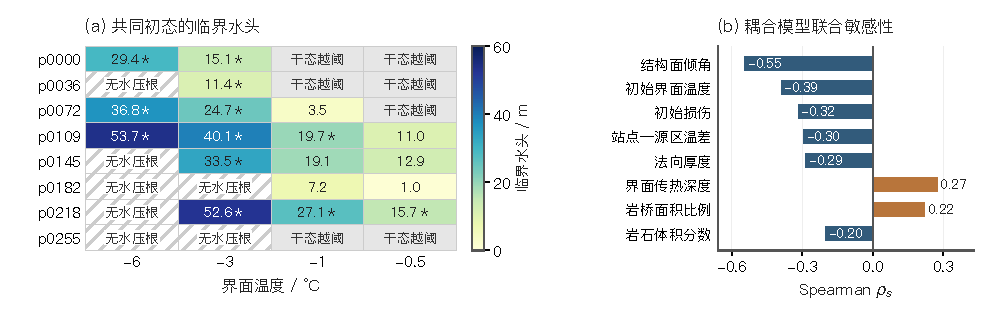
\includegraphics[width=\linewidth]{figures/q2/q2_critical_head_sensitivity.pdf}
\caption{条件临界水头与耦合敏感性。左图取八个固定初始损伤的设计代表；星号表示正根超出连通容量，斜线格无单独水压根，灰格为干态已临界。右图为解析热 STH 线性分支中评估期最小裕度的联合设计 Spearman 关联。}
\label{q2:fig-critical}
\end{figure}

\subsection{共同设计的机制比较与数值支持}\label{q2:sec-results}

表\ref{q2:tab-mechanisms}汇总解析热线性强度分支。相同结构基础下，开启内部热路径使后续越阈设计点由 4 增至 28，单独水力路径为 6，耦合路径为 31；相应评估期最小裕度中位数由 0.6901 降至 0.4718。热路径在该参数域改变更多设计点的稳定状态，水力路径则通过有效应力和损伤反馈进一步调节临界接近程度。

\begin{table}[htbp]
\centering\small
\caption{解析热线性强度分支的共同设计结果，每行 256 点}
\label{q2:tab-mechanisms}
\begin{tabular}{@{}lrrrr@{}}
\toprule
机制 & 后续越阈 & 初始左删失 & 未越阈 & 最小裕度中位数\\
\midrule
S & 4 & 31 & 221 & 0.6901\\
ST & 28 & 31 & 197 & 0.4853\\
SH & 6 & 31 & 219 & 0.6623\\
STH & 31 & 31 & 194 & 0.4718\\
\bottomrule
\end{tabular}
\par\smallskip\footnotesize 越阈分类覆盖全计算期；最小裕度取 8 月 19--27 日。设计点计数和分位数描述条件参数域，不赋予事件概率；本地独立灾害验证事件数为 0。
\end{table}

\begin{figure}[htbp]
\centering
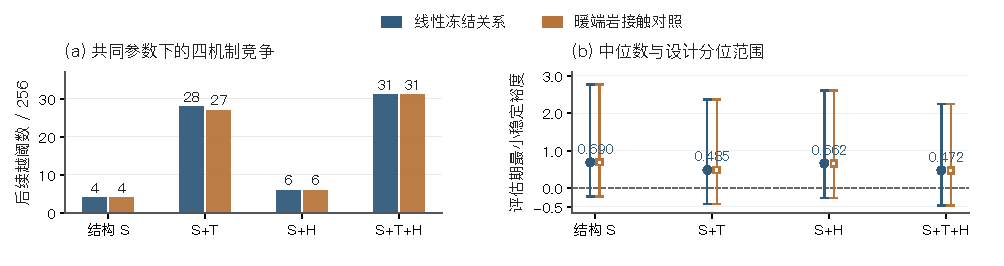
\includegraphics[width=\linewidth]{figures/q2/q2_mechanism_comparison.pdf}
\caption{四机制在相同设计下的越阈与稳定裕度响应；两种暖端强度策略并列，区间表示设计点的 5\%--95\% 分位。}
\label{q2:fig-mechanisms}
\end{figure}

两强度策略合计得到 137 个后续越阈、248 个初始左删失和 1663 个未越阈情景。暖端接触策略仅将 ST 的后续越阈数由 28 改为 27，其余组计数相同。图\ref{q2:fig-critical}的联合设计中，STH 最小裕度与倾角、初温、初损伤、站源温差、厚度的相关系数依次约为 $-0.545$、$-0.390$、$-0.318$、$-0.296$、$-0.285$；这些方向说明较陡、较暖及较高初损伤的条件更接近临界，排序随规定参数范围解释。

解析热与 0.0625 m 有限差分参考的 137 个有限时刻配对中，最大越阈时间差为 0.347 h，类别保持一致；与 0.125 m 网格的最大差为 19.0724 h。因而本文以解析热作为所声明线性导热问题的参考，同时保留小时水量和损伤更新的离散支持。暖端不连续切换仍可造成最大裕度差 0.1790，热模块精度与整体机械时刻精度分别讨论。

在本设计的深度、扩散率和边界序列下，将半无限解与 40 m 无通量底边界比较，边界总变差乘首反射核得到的最大温差界为 $2.38\times10^{-26}\,^{\circ}\mathrm C$。因此这一计算期内的理想底边界选择影响很小，现场解释主要依赖表面映射、初始热状态以及裂隙水热输运等过程条件。

进一步对岩桥强度、损伤、水头、温度四未知量作局部雅可比分析，单裕度、同条件重复裕度、增添温度、温度加压力、再增理想损伤观测时的秩依次为 $1,1,2,3,4$。这一结果将监测重点指向同一结构面的温压与岩桥损伤联合约束，而非仅增加相同条件下的采样次数。

\subsection{暖域高应力的外部本构挑战}\label{q2:sec-laboratory}

为检验式\eqref{q2:eq-strength}的应力迁移，本文完整读取官方补充表的 141 次试验和 14 条派生温层摘要，后者用于作者关系复核，逐试验数据用于新拟合。名义 800 kPa 组有 20 次试验，面积修正后实测应力为 808.89--868.63 kPa；其温度设计仅覆盖 $-4$ 至 $-0.5\,^{\circ}\mathrm C$。按名义温应力组划分数据，拟合使用破坏时实测列，保留重复标签的身份歧义和相关性敏感性。

四种固定候选在四域、两权重下形成 32 个拟合、576 个整组留出折。五暖温层的全应力共同域含 83 次试验；图\ref{q2:fig-lab}按整温层、整应力层比较跨条件泛化。温度线性 MC 的训练 RMSE 为 187.45 kPa，两类留出的组等权宏 RMSE 为 198.41、296.34 kPa。应力二次和 400 kPa 铰链虽将训练误差降至 174.32、177.41 kPa，仅留 800 组时却分别增至 925.78、2065.13 kPa，显示高应力分支外推的敏感性。

\begin{table}[htbp]
\centering\small
\caption{共同暖域本构复杂度与应力层外推误差（kPa）}
\label{q2:tab-lab}
\begin{tabular}{@{}lrrr@{}}
\toprule
候选 & 参数数 & 训练 RMSE & 仅留 800 组 RMSE\\
\midrule
温度线性 MC & 4 & 187.45 & 443.94\\
温度二次 MC & 6 & 185.39 & 421.07\\
应力二次 & 6 & 174.32 & 925.78\\
400 kPa 铰链 & 6 & 177.41 & 2065.13\\
\bottomrule
\end{tabular}
\par\smallskip\footnotesize 主权重为逐试验 OLS；仅留 800 组时，其余 63 次暖域试验训练、20 次高应力试验评价。
\end{table}

\begin{figure}[htbp]
\centering
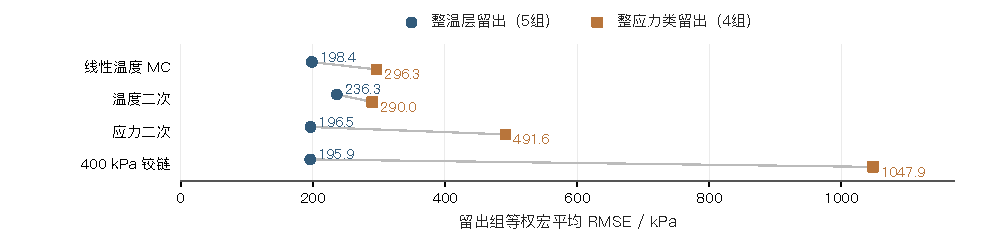
\includegraphics[width=\linewidth]{figures/q2/q2_lab_grouped_validation.pdf}
\caption{83 次暖域外部试验的分组留出比较。宏 RMSE 为各折 RMSE 平方的等权均值再开方；作者 Eq6 另作描述性复核，不纳入留出比较。}
\label{q2:fig-lab}
\end{figure}

作者在共同暖域内的低应力与全应力拟合分别选取三、四个显著温层，因此系数变化同时包含应力覆盖与筛温影响。本文另以完整五暖层进行比较，保留温度线性 MC 作为低复杂度外部挑战；本地计算继续使用原式与原版本。条件 bootstrap 均值范围、试验重复相关性和跨材料迁移分别记录，外部试验数不加入本地灾害验证分母。
以原实验的名义坐标 $T=-2\,^{\circ}\mathrm C$、$\sigma=800$ kPa 为例，暖域线性 MC 的条件均值为 659.30 kPa；单元内逐试验与整标签重采样的均值 2.5\%--97.5\% 分位范围分别为 614.49--714.29、607.58--691.88 kPa。

八个重复标签的物理试件映射保持未知，两种方案用于展示相关结构敏感性；这些范围描述给定模型下的均值变动，个体散差与现场迁移另作解释。

综上，结构水热框架给出了从气象输入到界面状态、稳定裕度和条件临界水头的完整链条。STH 用于统一状态推进，S、ST、SH 用于辨别传递路径；源区首次机械越阈与整体释放、下游到达分别交接。该设计将机制比较与后续时刻预测相联，并将最有价值的新增观测明确为界面温度、连通水压和岩桥损伤信息。
\AIcredit
